\section{Исследование и построение решения задачи}
\label{sec:Chapter3} \index{Chapter3}

% Требуется разбить большую задачу, описанную в постановке, на более мелкие
% подзадачи. Процесс декомпозиции следует продолжать до тех пор, пока подзадачи
% не станут достаточно простыми для решения непосредственно. Это может быть
% достигнуто, например, путем проведения эксперимента, доказательства теоремы
% или поиска готового решения.

Самые распространённые гонки, встречающиеся в реальных проектах, можно разделить на три категории. Далее, по ходу их рассмотрения, будут предложены алгоритмы для их автоматического обнаружения.

\subsection{Гонка на содержимом файла}

\lstinputlisting[
	caption={Пример Makefile с гонкой на содержимом объектных файлов},
    language=bash,
    label=lst:race-condition-1,
    escapechar=\%,
    morekeywords={all, write_a, append_b}
]{src/file-content-race-1.make}

В этом примере между целями \texttt{compile} и \texttt{link} не хватает зависимости. Аналогично примеру из вступления, при многопоточной сборке цель \texttt{link} может попытаться скомпоновать объектные файлы, которых ещё не существует, или использовать старый, ещё не обновленный объектный файл.

Основная идея автоматического обнаружения гонок заключается в отслеживании операций с файлами и сопоставление их с графом зависимостей системы сборки. Самый простой способ увидеть, как процесс работает с файлами --- запустить его под утилитой strace.

\lstinputlisting[
	caption={Фрагмент лога strace при сборке Makefile из листинга \ref{lst:race-condition-1}},
]{src/strace-log.txt}

В фрагменте полученного лога можно видеть, как процесcы 1017, 1020 и 1025 открывают одни и те же объектные файлы с помощью системного вызова \texttt{openat}, причём первые два --- на запись, а последний --- на чтение. Однако этой информации мало: из лога нельзя понять, какие цели сборки скрываются за этими номерами.

Чтобы сопоставить номера процессов с целями сборки предлагается модифицировать саму утилиту Make. В качестве подопытного был взят проект remake. Он реализует тот же функционал, что и GNU Make, но требует значительно меньше усилий для сборки из исходного кода. После внесения изменений (см. приложение \ref{subsec:remake-patch}) в логе сборки появятся строки с информацией о том, какие процессы порождаются Make, и каким целям они соответствуют.

\lstinputlisting[
    label=lst:log-detailed,
	caption={Фрагмент лога сборки Makefile из листинга \ref{lst:race-condition-1} с модифицированным remake},
    language=bash,
    morekeywords={all, write_a, append_b}
]{src/strace-log-with-make-patch.txt}

Можно заметить, что ни один процесс \texttt{gcc}, запускается Make, не работает с файлами проекта напрямую. GCC --- не компилятор, а драйвер, который запускает нужные компиляторы и компоновщики. Создание \texttt{main.o} и \texttt{lib.o} ведётся дочерними процессами \texttt{gcc}. В нашем случае это процессы \texttt{as}, порождённые системным вызовом \texttt{vfork}. Они генерируют объектные файлы на основе ассемблера, в который компилируется Си с помощью \texttt{cc1} - другого дочернего процесса \texttt{gcc}.

\begin{figure}[H]
	\caption{Дерево процессов при сборке Makefile из листинга \ref{lst:race-condition-1}}
	\centering
	\begin{tikzpicture}
        \node[style=draw, minimum width=4cm] (compile) at (0,2.25) {Цель \texttt{compile}};
        \node[style=draw, minimum width=4cm] (link) at (0,0) {Цель \texttt{link}};

        \node[style=draw] (gcc3) at (5.5,0) {\parbox{4.5cm}{\centering \texttt{gcc main.o lib.o} \\ \footnotesize pid=1023}};
        \node[style=draw] (gcc1) at (5.5,3) {\parbox{4.5cm}{\centering \texttt{gcc main.cpp} \\ \footnotesize pid=1015}};
        \node[style=draw] (gcc2) at (5.5,1.5) {\parbox{4.5cm}{\centering \texttt{gcc lib.cpp} \\ \footnotesize pid=1018}};

        \node[style=draw] (ld) at (11,0) {\parbox{2.5cm}{\centering \texttt{ld} \\ \footnotesize pid=1025}};
        \node[style=draw] (as1) at (11,3) {\parbox{2.5cm}{\centering \texttt{as} \\ \footnotesize pid=1017}};
        \node[style=draw] (as2) at (11,1.5) {\parbox{2.5cm}{\centering \texttt{as} \\ \footnotesize pid=1020}};

        \draw[line width=1pt, shorten >=2pt, shorten <=2pt, ->] (compile) -- (gcc1);
        \draw[line width=1pt, shorten >=2pt, shorten <=2pt, ->] (compile) -- (gcc2);

        \draw[line width=1pt, shorten >=2pt, shorten <=2pt, ->] (gcc1) -- (as1) node[midway, above] {vfork};
        \draw[line width=1pt, shorten >=2pt, shorten <=2pt, ->] (gcc2) -- (as2) node[midway, above] {vfork};

        \draw[line width=1pt, shorten >=2pt, shorten <=2pt, ->] (link) -- (gcc3);
        \draw[line width=1pt, shorten >=2pt, shorten <=2pt, ->] (gcc3) -- (ld) node[midway, above] {vfork};
    \end{tikzpicture}
    \label{fig:pstree1}
\end{figure}

Схему выше (кроме названий процессов) можно построить на данных из листинга \ref{lst:log-detailed}. В ней, как и в фрагменте лога, опущены процессы \texttt{cc1}, поскольку они не производят доступов к интересующим нас объектным файлам.

Рассмотрим процессы 1020 и 1025. Из схемы выше, им соответствуют цели \texttt{compile} и \texttt{link} соответственно. В то же время из фрагмента лога \ref{lst:log-detailed} можно установить, что процесс 1020 производит запись в файл \texttt{lib.o}, а процесс 1025 - чтение того же файла. Запись в файл и чтение файла нельзя менять местами, иначе результат чтения может измениться. Следовательно процессы 1020 и 1025 должны запускаться строго друг за другом. Иными словами, между соответствующими целями --- \texttt{compile} и \texttt{link} должна быть зависимость. Проверим это, обратившись к графу зависимостей схемы.

\begin{figure}[H]
	\caption{Граф зависимостей Makefile из листинга \ref{lst:race-condition-1}}
	\centering
	\begin{tikzpicture}[every node/.style = draw]
        \node[inner xsep=7pt] (link) at (0,0) {link};
        \node[inner xsep=7pt] (compile) at (0,1.2) {compile};
        \node[inner xsep=7pt] (all) at (3,0.6) {all};


        \draw[line width=1pt, shorten >=2pt, shorten <=2pt, <->] (link) -- (compile);
        \draw[line width=1pt, -] (-0.2,0.5) -- (0.2,0.7);
        \draw[line width=1pt, -] (0.2,0.5) -- (-0.2,0.7);

        \graph {
            (link) ->[line width=1pt, shorten >=2pt, shorten <=2pt] (all);
            (compile) ->[line width=1pt, shorten >=2pt, shorten <=2pt] (all);
        };
    \end{tikzpicture}
\end{figure}

Легко убедиться в том, что схема сборки из примера не содержит такой зависимости: между целями \texttt{link} и \texttt{compile} нет ориентированного пути. Соответственно, в схеме сборки присутствует гонка. Теперь можно составить первый вариант алгоритма автоматического поиска состояний подобных гонок:

\begin{enumerate}
	\item Произвести сборку с использованием strace и модифицированного remake;
	\item Получить соответствие между pid и целями сборки;
	\item Получить список доступов к файлам для каждой известной цели;
	\item Найти конфликтующие доступы к одному и тому же пути из разных целей;
	\item Убедиться в том, что в схеме сборки существуют зависимости между целями, производящими конфликтующие доступы;
\end{enumerate}

В таком виде у алгоритма есть одно ограничение. Если цели \texttt{compile} и \texttt{link} будут использовать жёсткие ссылки на объектные файлы (например, \texttt{main.o.0} и \texttt{main.o.1}), гонка останется, но в логе доступов будут фигурировать пути от разных жёстких ссылок. Алгоритм выше не обнаружит такую гонку, поскольку полагается на совпадение путей как строк. Вместо этого нужно использовать какой-то другой способ сравнения, который бы учитывал жесткие ссылки.

В системе Linux у каждого файла или директории существует ассоцированная с ним index node (inode). Получить её номер из поля \texttt{st\_ino} структуры \texttt{stat}. Согласно стандарту ядра, жесткие ссылки внутри одной файловой системы ссылаются на одну и ту же inode \cite{inode-docs}. Если речь идёт о нескольких файловых системах, то потребуется обратить внимание ещё и на device number (поле \texttt{st\_dev} из той же структуры \texttt{stat}). В разработанном инструменте это учтено, однако для простоты далее в этой работе device number будет опускаться.

Номера inode могут быть переиспользованы системой, когда все жесткие ссылки на файл оказываются удалены. Это может привести к тому, что разные файлы будут отражены в логе одними и теми же номерами inode, в результате чего алгоритм выдаст ложные срабатывания. Если добавить в лог события освобождения inode, скрипт для поиска гонок сможет отличать их поколения, и не выдавать ложных срабатываний при переиспользовании inode.

Прежде наш алгоритм полагался на парсинг лога strace. К сожалению, эта утилита не позволяет производить такие сложные проверки. Для этой цели лучше подходит \texttt{ptrace} --- системный вызов для трассировки процессов, на основе которого реализован отладчик GDB, а так же сам strace. \texttt{ptrace} позволяет перехватывать управление процессом перед любыми системными вызовами, которые он совершает. Таким образом, можно заменить звено strace на собственный трассировщик на основе \texttt{ptrace}. Он позволить производить более сложные проверки и составлять более информативные логи.

Перехватив управление процессом перед удалением файла или директории (системные вызовы \texttt{unlink(at)} или \texttt{rmdir}), трассировщик может проверить, что оно приведёт к освобождению номера inode. Linux указывает количество жестких ссылок на файл в поле \texttt{st\_nlink} структуры \texttt{stat}. Перед удалением последней жёсткой ссылки (и, соответственно, перед освобождением номера inode) \texttt{st\_nlink} равняется 1 для файлов и 2 для директорий (каждая директория содержит <<\texttt{.}>> --- жесткую ссылку на себя). Произведя такую проверку, трассировщик сможет вывести в лог событие освобождения номера inode.

Таким образом, после всех исправлений, алгоритм приобретает следующий вид:

\begin{enumerate}
	\item Произвести сборку с использованием модифицированного remake и трассировщика на Си, использующего \texttt{ptrace};
	\item Получить соответствие между pid и целями сборки;
	\item Получить список доступов к inode для каждой известной цели;
	\item Найти конфликтующие доступы к одному и тому же поколению inode из разных целей;
	\item Убедиться в том, что в схеме сборки существуют зависимости между целями, производящими конфликтующие доступы к одному и тому же поколению inode;
\end{enumerate}

\subsection{Гонка на пути к файлу}

\lstinputlisting[
	caption={Пример Makefile с гонкой на пути к файлу},
    label=lst:race2,
	language=bash,
]{src/file-path-race-3.make}

В предыдущей главе мы строили алгоритм для ситуации, в которой гонка происходит на содержимом одного и того же файла. Здесь же речь пойдёт о разных файлах, которые были доступны по одному и тому же пути в разные моменты времени. В листинге \ref{lst:race2} представлен распространённый сценарий гонки: независимые цели \texttt{something} и \texttt{something\_else} выбрали одно и то же имя для своих временных файлов. Если бы сборка этих целей была запущена параллельно, то мог бы возникнуть конфликт.

Значительная часть предыдущей главы была уделена борбье с жесткими ссылками. Это связано с тем, что файл может иметь несколько абсолютных путей. Для директорий это неверно, поскольку целью жестких ссылок могут быть только файлы (за исключением <<.>> и <<..>>, которые не используются в абсолютных путях). Следовательно, для директорий корректно использовать их абсолютные пути в качестве уникального идентификатора. Стоит оговориться, что для этого нужно использовать разрешённый путь, то есть не содержащий переходов по символическим ссылкам. Далее под путями будут подразумеваться абсолютные разрешенные пути.

Если в некоторой директории $d$ два разных файла были доступны по имени $n$ в разные моменты времени, это означает, что между этим было произведено удаление и повторное создание этого файла. Поскольку к этой директории существует единственный путь, его удаление и создание не могло быть произведено ни по какому пути, кроме $d$/$n$. Следовательно, для поиска таких гонок достаточно искать зависимости между целями, которые удаляют и создают файлы по одному и тому же пути. В этом случае пользоваться номерами inode уже не нужно.

\subsection{Гонка между созданием директории и файла внутри неё}

\lstinputlisting[
	caption={Пример Makefile с гонкой третьей категории},
	label=lst:race3,
    language=bash,
]{src/directory-race-4.make}

В листинге \ref{lst:race3} цели \texttt{build} и \texttt{build/a.out} не зависят друг от друга. Если цель \texttt{build/a.out} начнёт собираться раньше, она не сможет создать файл в директории, которой ещё не существует. Такая гонка была обнаружена в проекте GPM с помощью \texttt{make {-}{-}shuffle} \cite{race-3-example}. Предыдущие алгоритмы не помогут в поиске таких гонок.

Директория и файл внутри неё --- разные элементы файловой системы, имеющие разные пути и разные номера inode, поэтому предыдущие алгоритмы не смогут обнаружить эту гонку. Простое решение --- фиксировать доступ специального вида (directory lookup) к родительской папке при любом обращении к лежащему в ней файлу.

% \begin{figure}[H]
%     \caption{Операции над файлами при сборке Makefile из листинга \ref{lst:race3}}
%     \centering
%     \begin{tikzpicture};
%         \node at (4.5,5) {Процессы:};
%         \node at (12,5) {Доступы:};

%         \node[style=draw, minimum width=3cm, minimum height=0.9cm] (mkdir) at (4.5,3) {\texttt{mkdir build}};
%         \node[style=draw, minimum width=3cm, minimum height=1.9cm] (echo) at (4.5,1.5) {\texttt{echo ...}};

%         \node at (10,4) {\texttt{./build}};
%         \node at (14,4) {\texttt{./build/a.out}};

%         \node[minimum width=4cm, minimum height=1cm] (dirwrite) at (10,3) {\texttt{write}};
%         \node[minimum width=4cm, minimum height=1cm] (dirlookup) at (10,2) {\texttt{dir\_lookup}};
%         \node[minimum width=4cm, minimum height=1cm] (filewrite) at (14,1) {\texttt{write}};

%         \draw[->, shorten >=4pt, shorten <=4pt] (mkdir) to[out=0, in=180] (dirwrite);
%         \draw[->, shorten >=4pt, shorten <=4pt] ($(echo.north east)!0.2375!(echo.south east)$) -- (dirlookup);
%         \draw[->, shorten >=4pt, shorten <=4pt] ($(echo.north east)!0.7625!(echo.south east)$) -- (filewrite);

%         \draw[thick] (8,0) -- (8,4.3);
%         \draw[thick] (12,0) -- (12,4.3);
%         \draw[thick] (16,0) -- (16,4.3);
%         \draw[thick] (8.5,3.5) -- (11.5,3.5);
%         \draw[thick] (12.5,3.5) -- (15.5,3.5);

%         \node[gray, font=\itshape] (time) at (2, -0.5) {$\tau$};
%         \draw[gray, line width=0.7pt, ->] (2, 4.3) to (2, 0);
%     \end{tikzpicture}
%     \label{fig:dirlookup-demo}
% \end{figure}

\begin{figure}[H]
    \caption{Операции над файлами при сборке Makefile из листинга \ref{lst:race3}}
    \centering
    \begin{tikzpicture};
        \node at (3.5,4) {Процессы:};
        \node at (12,4) {Файловая система:};

        \node[style=draw, minimum width=5cm, minimum height=0.9cm] (mkdir) at (3.5,3) {\texttt{mkdir build}};
        \node[style=draw, minimum width=5cm, minimum height=1.9cm] (echo) at (3.5,1.5) {\texttt{echo > build/a.out}};

        \node[align=left, text width=3cm] (build) at (12.5,3) {\texttt{./build}};
        \node[align=left, text width=3cm] (buildaout) at (12.5,1) {\texttt{./build/a.out}};

        \draw[->, shorten >=4pt, shorten <=4pt] (6,3) -- (11,3);
        \draw[-, shorten <=4pt] (6,2) -- (9,2);
        \draw[->, shorten >=4pt] (9,2) to[in=180, out=0] (11,3);
        \draw[->, shorten >=4pt, shorten <=4pt] (6,1) -- (11,1);

        \node at (7.7, 3.3) {\texttt{write}};
        \node at (7.7, 2.3) {\texttt{dir\_lookup}};
        \node at (7.7, 1.3) {\texttt{write}};

        \node[gray, font=\itshape] (time) at (0.5, 0.5) {$\tau$};
        \draw[gray, line width=0.7pt, ->] (0.5, 4) to (0.5, 1);
    \end{tikzpicture}
    \label{fig:dirlookup-demo}
\end{figure}

Операция \texttt{dir\_lookup} позволила связать процесс \texttt{echo} из цели \texttt{build/a.out} с процессом \texttt{mkdir} из цели \texttt{build}. Поскольку теперь они производят чтение и запись на одной и той же директории, алгоритм поиска гонок из первой главы проверит наличие зависимости между их целями. Несмотря на то, что доступ \texttt{dir\_lookup} фиксируется только к ближайшему родительскому каталогу, этот принцип применим и для большего числа вложенных директорий.

\begin{figure}[H]
    \caption{Операции над файлами для большего числа вложенных директорий}
    \centering
    \begin{tikzpicture};
        \node at (3,6) {Процессы:};
        \node at (12,6) {Файловая система:};

        \node[style=draw, minimum width=6cm, minimum height=0.9cm] (mkdir) at (3,5) {\texttt{mkdir build}};
        \node[style=draw, minimum width=6cm, minimum height=1.9cm] (mkdir) at (3,3.5) {\texttt{mkdir build/foo}};
        \node[style=draw, minimum width=6cm, minimum height=1.9cm] (echo) at (3,1.5) {\texttt{echo > build/foo/a.out}};

        \node[align=left, text width=3cm] (build) at (12.5,5) {\texttt{./build}};
        \node[align=left, text width=3cm] (buildfoo) at (12.5,3) {\texttt{./build/foo}};
        \node[align=left, text width=3cm] (buildfooaout) at (12.5,1) {\texttt{./build/foo/a.out}};

        \draw[->, shorten >=4pt, shorten <=4pt] (6,3) -- (11,3);
        \draw[-, shorten <=4pt] (6,2) -- (9,2);
        \draw[->, shorten >=4pt] (9,2) to[in=180, out=0] (11,3);
        \draw[->, shorten >=4pt, shorten <=4pt] (6,1) -- (11,1);

        \draw[->, shorten >=4pt, shorten <=4pt] (6,5) -- (11,5);
        \draw[-, shorten <=4pt] (6,4) -- (9,4);
        \draw[->, shorten >=4pt] (9,4) to[in=180, out=0] (11,5);

        \node at (7.7, 5.3) {\texttt{write}};
        \node at (7.7, 4.3) {\texttt{dir\_lookup}};
        \node at (7.7, 3.3) {\texttt{write}};
        \node at (7.7, 2.3) {\texttt{dir\_lookup}};
        \node at (7.7, 1.3) {\texttt{write}};

        \node[gray, font=\itshape] (time) at (-0.5, 0.5) {$\tau$};
        \draw[gray, line width=0.7pt, ->] (-0.5, 6) to (-0.5, 1);
    \end{tikzpicture}
    \label{fig:dirlookup-demo-deep}
\end{figure}

При создании множественных вложенных директорий, доступ \texttt{dir\_lookup} связывает между собой все <<соседние>> процессы. Если окажется, что все процессы, которые создают цепочку вложенных директорий, связаны соотвествующей цепочкой зависимостей, то гонки будут исключены. Верно и обратное: если, например, \texttt{mkdir build} и \texttt{mkdir build/foo} не связаны зависимостью (цепочка зависимостей разорвана), то присутствует гонка --- вторая цель может исполниться раньше первой, что приведёт к ошибке.

%  При доступе цели к какому-либо файлу он будет требовать от неё наличия зависимости с той целью, которая создала содержащий его каталог.

Однако на практике этот алгоритм часто выдаёт ложные срабатывания. Проблема в том, что хоть две записи в файл и являются критическими операциями (поскольку влияют на содержимое файла) и требуют наличия зависимости, две попытки создания одной и той же директории могут быть безопасно переставлены местами. Результат не поменяется --- директория всё равно будет создана в тот же момент времени.

\lstinputlisting[
    caption={Пример Makefile с созданием директории build из нескольких целей},
    label=lst:race3-complex,
    language=bash,
]{src/directory-race-5.make}

В Makefile, изображённом на листинге \ref{lst:race3-complex}, несколько целей самостоятельно создают папку \texttt{build}, а затем используют её для сборки. Предложенный выше алгоритм выдаст ложные срабатывания, зафиксировав первую цель \texttt{libN}, которая первая создала директорию \texttt{build}, и ошибочно потребовав от всех остальных целей \texttt{lib(M $\ne$ N)} иметь зависимость с \texttt{libN}.

В корректированной версии алгоритма операция \texttt{dir\_access} должна требовать наличие зависимости не с единственным успешным созданием директории, а хотя бы с одной, любой попыткой это сделать. Для этого нужно также модифицировать трассировщик системных вызовов: он должен сообщать о тех \texttt{mkdir}, которые завершились с \texttt{EEXIST}. Если для наглядности добавить в схему из листинга \ref{lst:race3-complex} десятую библиотеку, которая не делает \texttt{mkdir -p build}, новый алгоритм найдёт её и корректно сообщит о гонке.

\begin{figure}[H]
    \centering
    \caption{Обнаружение гонок на основе попыток создания директории}
    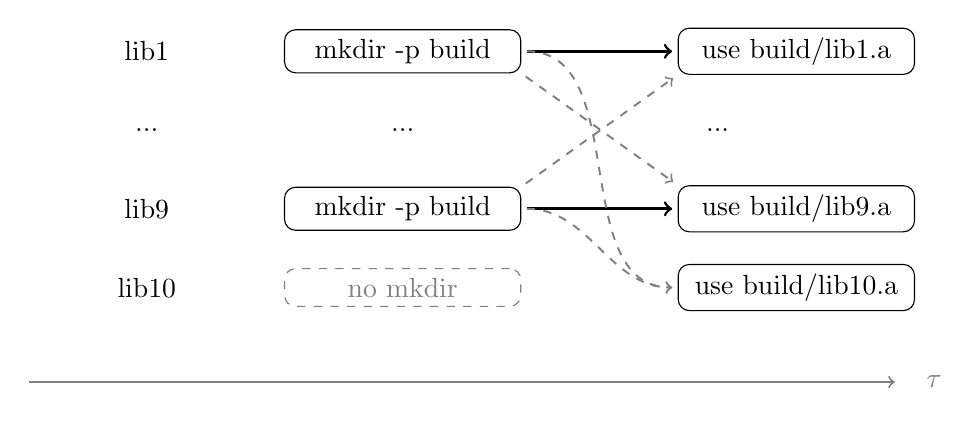
\begin{tikzpicture}
        % Common
        \node[style=draw, rounded corners, minimum width=3cm] (lib1build) at (3.75,2) {mkdir -p build};
        \node[style=draw, rounded corners, minimum width=3cm] (lib1) at (8.75,2) {use build/lib1.a};

        \node at (3.75,1) {...};
        \node at (7.75,1) {...};

        \node[style=draw, rounded corners, minimum width=3cm] (lib9build) at (3.75,0) {mkdir -p build};
        \node[style=draw, rounded corners, minimum width=3cm] (lib9) at (8.75,0) {use build/lib9.a};

        \node at (0.5,2) {lib1};
        \node at (0.5,1) {...};
        \node at (0.5,0) {lib9};

        % Time text and arrow
        \node[gray, font=\itshape] (time) at (10.5, -2.2) {$\tau$};
        \draw[gray, line width=0.7pt, ->] (-1, -2.2) to (10, -2.2);

        \draw[line width=1pt, shorten >=2pt, shorten <=2pt, ->] (lib1build) -- (lib1);
        \draw[line width=1pt, shorten >=2pt, shorten <=2pt, ->] (lib9build) -- (lib9);
        \draw[gray, dashed, line width=0.7pt, shorten >=2pt, shorten <=2pt, ->] (lib1build.south east) -- (lib9.north west);
        \draw[gray, dashed, line width=0.7pt, shorten >=2pt, shorten <=2pt, ->] (lib9build.north east) -- (lib1.south west);

        \node[style=draw, rounded corners, minimum width=3cm] (lib10) at (8.75,-1) {use build/lib10.a};
        \node at (0.5,-1) {lib10};
        \node[gray, style=draw, rounded corners, dashed, minimum width=3cm] (lib10build) at (3.75,-1) {no mkdir};
        \draw[gray, dashed, line width=0.7pt, shorten >=2pt, shorten <=2pt, ->] (lib1build) to[out=0, in=180] (lib10);
        \draw[gray, dashed, line width=0.7pt, shorten >=2pt, shorten <=2pt, ->] (lib9build) to[out=0, in=180] (lib10);
    \end{tikzpicture}
\end{figure}

